%\documentclass[PhD]{iitmdiss}
%\documentclass[MS]{iitmdiss}
%\documentclass[MTech]{iitmdiss}
\documentclass[BTech]{iitmdiss}
\usepackage{times}
 \usepackage{t1enc}
 
\newcommand{\source}[1]{\caption*{Source: {#1}} }
\usepackage{graphicx}
\usepackage{caption}
\usepackage{epstopdf}
\usepackage[hypertex]{hyperref} % hyperlinks for references.
\usepackage{amsmath} % easier math formulae, align, subequations \ldots
\usepackage{listings}
\usepackage{color}
 
\definecolor{codegreen}{rgb}{0,0.6,0}
\definecolor{codegray}{rgb}{0.5,0.5,0.5}
\definecolor{codepurple}{rgb}{0.58,0,0.82}
\definecolor{backcolour}{rgb}{0.95,0.95,0.92}
 
\lstdefinestyle{mystyle}{
    backgroundcolor=\color{backcolour},   
    commentstyle=\color{codegreen},
    keywordstyle=\color{magenta},
    numberstyle=\tiny\color{codegray},
    stringstyle=\color{codepurple},
    basicstyle=\footnotesize,
    breakatwhitespace=false,         
    breaklines=true,                 
    captionpos=b,                    
    keepspaces=true,                 
    numbers=left,                    
    numbersep=5pt,                  
    showspaces=false,                
    showstringspaces=false,
    showtabs=false,                  
    tabsize=2
}


\begin{document}

%%%%%%%%%%%%%%%%%%%%%%%%%%%%%%%%%%%%%%%%%%%%%%%%%%%%%%%%%%%%%%%%%%%%%%
% Title page

\title{ RB-Tree Implementation on GPU}

\author{Rohith Kumar Miryala}

\date{April 2016}
\department{COMPUTER SCIENCE AND ENGINEERING}

%\nocite{*}
\maketitle

%%%%%%%%%%%%%%%%%%%%%%%%%%%%%%%%%%%%%%%%%%%%%%%%%%%%%%%%%%%%%%%%%%%%%%
% Certificate
\certificate

\vspace*{0.5in}

\noindent This is to certify that the thesis titled {\bf RB-tree Implementation on GPU}, submitted by {\bf Rohith Miryala}, 
  to the Indian Institute of Technology, Madras, for
the award of the degree of {\bf B.tech}, is a bona fide
record of the research work done by him under our supervision.  The
contents of this thesis, in full or in parts, have not been submitted
to any other Institute or University for the award of any degree or
diploma.

\vspace*{1.5in}

\begin{singlespacing}
\hspace*{-0.25in}
\parbox{2.5in}{
\noindent {\bf Prof. ~Rupesh ~Nasre} \\
\noindent Research Guide \\ 
\noindent Dept. of Computer Science and Engineering\\
\noindent IIT-Madras, 600 036 \\
} 
\hspace*{1.0in} 
%\parbox{2.5in}{
%\noindent {\bf Prof.~S.~C.~Rajan} \\
%\noindent Research Guide \\ 
%\noindent Assistant Professor \\
%\noindent Dept.  of  Aerospace Engineering\\
%\noindent IIT-Madras, 600 036 \\
%}  
\end{singlespacing}
\vspace*{0.25in}
\noindent Place: Chennai\\
Date: 24th April 2016 


%%%%%%%%%%%%%%%%%%%%%%%%%%%%%%%%%%%%%%%%%%%%%%%%%%%%%%%%%%%%%%%%%%%%%%
% Acknowledgements
\acknowledgements

I am very thankful to my advisor Rupesh Nasre for letting me choose this project. He has been very encouraging and always helped me whenever I was stuck. I also thank Anurag Ingole who helped me in getting familiar with the OpenCL language.

%%%%%%%%%%%%%%%%%%%%%%%%%%%%%%%%%%%%%%%%%%%%%%%%%%%%%%%%%%%%%%%%%%%%%%
% Abstract

\abstract
\pagenumbering{arabic}
\vspace*{24pt}

\noindent Latest works show that GPU's have very high computing capability and they can be used for graph processing. The problem with GPU is dynamically updating graphs. Our goal is to implement RB-tree on GPU and compare the insertion times taken on CPU and GPU.

We used OpenCL and C languages for coding. Since OpenCL doesn't support dynamic allocation of memory on GPU, we prematurely assigned memory required for inserting nodes into RB-Tree. 

\pagebreak

%%%%%%%%%%%%%%%%%%%%%%%%%%%%%%%%%%%%%%%%%%%%%%%%%%%%%%%%%%%%%%%%%
% Table of contents etc.

\begin{singlespace}
\tableofcontents
\thispagestyle{empty}
\end{singlespace}

%%%%%%%%%%%%%%%%%%%%%%%%%%%%%%%%%%%%%%%%%%%%%%%%%%
% Introduction.

\chapter{INTRODUCTION}
\label{chap:intro}
\section{Trees}
Trees are used as Abstract Data Type(ADT) in Computer Science. Unlike Arrays which are linear, trees are hierarchical data structure.A tree data structure is defined using collection of nodes. Each node points to other nodes which are its children. In a binary tree,the number of children are limited to 2. Trees are implemented using linked lists. Each node has pointers to its children and parent.This makes searching easy.Using self balancing trees like AVL or RB-Trees, they provide a upper bound on the time taken for search.Since trees are hierarchical structures, they are used in file systems on computers which are hierarchical. Some common uses of trees are representing hierarchical data structures, storing information that makes it search-able, routing algorithms etc.\\
\section{RB-Trees}
RB-Trees are special kind of binary trees. They are self balancing trees. This self balancing property provides a upper bound on the search time taken. Each nodes has an extra bit to store the color of the node. Each node has either red color or black color.The tree is balanced using some constraints on these colors. The leaf nodes of RB-Trees do not contain data. They are used as sentinel nodes. Some algorithms use a single sentinel node. It has to be decided depending on the algorithm. Using a single node might save memory but affect performance. If different sentinel nodes are used, memory will be wasted. It has to be decided depending on the algorithm. Some real life applications of RB-Trees are, Completely Fair Scheduler in Linux kernel, C++ uses RB-Tree internally to implement set and map, data structures in computational geometry etc. \\
\section{Synchronization in Parallelization}
RB-Tree code needs to be parallalized to implement it on GPU. Data needs to be synchronized to run the code parallel. Millions of threads are spawned and each thread works on its nodes. While a thread is processing on a node, other thread should not be able to access the node to maintain data integrity. Locks have to be acquired on the nodes for synchronization. The locks have to be acquired atomically. If they are not acquired atomically, it might lead to dead lock or live lock.\\
A dead lock can occur when a thread acquires a lock and do not release the lock after it finished processing. In dead lock threads or blocked and unable to make any progress. Such conditions have to be taken care of.\\
A live lock can occur when a thread reacts to the action of other thread which in turn react to the action of this thread. In our algorithm, we will be acquiring the lock on 4 nodes. Live lock might occur when one thread acquires lock on two of nodes and other thread acquire lock on other two nodes. \\
Live lock can be avoided by taking locks in a particular order. Since both threads try to acquire locks on same node ,only one thread acquires a lock.\\
\section{Outline}
We will be looking at RB-trees in detail and how do we implement it. How to parallalize the code to implement it on GPU. What are experimental results and future work.

\chapter{Background}
\section{Red Black Trees}
Red Black Trees are binary search trees with colors attached to the nodes. By maintaining the invariants on node colors, the tree is always balanced. A red black tree has following properties\\
\begin{enumerate}  
\item Every node is either red or black
\item The root is black
\item Every Leaf(NIL) is black
\item If a node is red, then both its children are black
\item For each node, all simple paths from the node to descendant leaves contain the same number of black nodes
\end{enumerate} 
By maintaining this invariants, the tree is always balanced. A RB-Tree with n nodes has height at most 2lg(n+1). We prove this by induction. First define black height of node x as the number of black nodes from x to the leaf not including x. We denote this by bh(x). First we prove that a sub tree rooted at x has atleast $2^{bh(x)}-1$ internal nodes.We prove this claim by induction on height. If black height is 0, then the tree is leaf and it has 0 internal nodes $2^{bh(x)}-1$ = $2^{0}-1$ = 0 which is true. Now consider a internal node x which has 2 children. Each child has black height of bh(x) or bh(x)-1 depending on whether node x is red or black. Thus the subtree rooted at x has atleast $2^{bh(x)-1}-1$ + $2^{bh(x)-1}-1$ + 1 = $2^{bh(x)}-1 $ nodes. Let the height of the tree be h. The black height must be atleast h/2. Thus,\\
\begin{equation}
        n \ge 2^{h/2} - 1\\
\end{equation}
By taking logarithms on both sides we can yield\\
\begin{equation}
        h \le 2lg(n+1)\\
\end{equation}
Because of this many operations such as search, minimum, successor, predecessor all take O(lg(n)) time since each operation can be done in O(lg(h)) time. The two main operations of any tree is Insertion and Deletion of nodes. We see how do we restore the properties when a node is inserted or deleted.In our thesis, we will only be looking at insertion.\\
First we learn about rotations which are very useful in insertion and deletion. There are two types of rotations , Left Rotation and Right Rotation.
\subsection{Rotations}
\centerline{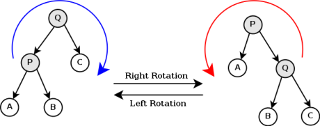
\includegraphics{treap-rotation.png}}
When we insert or delete a node, some properties of RB-Tree might be violated. To restore properties we change colors and also pointer structure of tree. We do this by using Rotations. Rotations preserve the binary search tree properties.\\
Doing a right rotation at Q made P as root and right child of P became the left child of Q and Q became the right child of P. We can see that binary search tree properties are preserved since Q value is greater than P, it is right child of P and B value is lesser than Q and it is left child of Q. Similarly left rotation can be done. When we do a right rotation on node x, we assume that its left child is not NULL since its left child becomes the new root. Similarly when we do a left rotation, its right child should not be NULL.
\subsection{Insertion}
A node can be inserted in O(lg(n)) time. A node is inserted similar to binary tree insertion. The inserted node is colored red. Now coloring the node red might violate one or more properties of RB-Tree. To restore the properties we call function RB-InsertFixup(). We will see wht properties can be violated because of coloring the new node red. Property 1 holds as color is red. Property 3 also holds as every node has 2 sentinel nodes which are black. Property 5 holds as we did not change the black nodes. So only property 2 and 4 can be violated. 2 is violated when inserted node is the root. This can be divided into 3 cases\\
\centerline{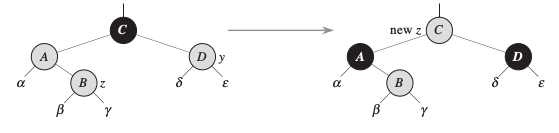
\includegraphics{cse1.png}}
\centerline{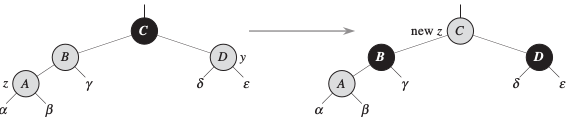
\includegraphics{case1.png}}\\
First case is z's uncle y is red. In this case we color both the nodes z's parent and uncle black and color grand parent to red.The algorithm is repeated with C as new z.\\
\centerline{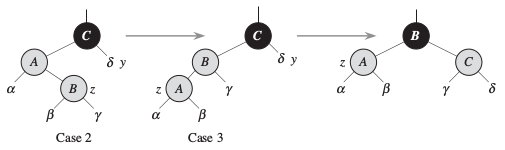
\includegraphics{case2,3.png}}\\
Case 2 is z's uncle y is black and z is a right child\\
Case 3 is z's uncle y is black and z is a left child\\
We can change the case 2 to case 3 by doing a left rotation on A. In case 3, B is colored black, C is colored red and a rotation is performed on C making B as root. The algorithm stops here.\\
*Images taken from Introduction to algorithms, Thomas Cormen, Charles Leierson, Ronald Rivest,  Clifford Stein.
\section{GPU and OpenCL}
Graphical Processing Unit(GPU) are high end computing devices. GPU's are used in phones, computers, gaming consoles adn embedded systems. GPU's are especially designed to do SIMD operations effectively. Initially GPU's are used for 3d graphic rendering, later extended to geometric calculations such as rotations and translating vertices to different coordinate systems. GPU's are suited for parallel problems. Atomic operations are possible in GPU at hardware level which are very fast compared to CPU. Hence scientists started studying GPU's for non graphical problems.\\
Open Computing Language(OpenCL) is a framework to code parallel programs which can be executed across many platforms. OpenCL supports CPU, GPU, FPGA and digital signal processing. Unlike CUDA which is specifically designed for Nvidia GPU, OpenCL supports both Nvidia and Radeon GPU's. OpenCL is based on C99 language.OpenCL views CPU and GPU as computing devices. OpenCL launches a kernel which can be run on any computing device. GPU's have separate memory. Hence pointers on host and GPU are not same. The data structures on host side are sent to kernel using arrays. Tree pointer cannot be sent directly to kernel. Hence a different data structure has to be chosen to implement the tree.



\chapter{Parallel RB-trees on GPU}
A parallel version of RB-Trees is implemented in synchrobench which is a micro-benchmark suite used to evaluate synchronization techniques on data structures.Synchrobench uses transactional memory operations to implement in parallel. The program runs on CPU. Now we want to implement it on GPU. Standard algorithms use linked lists to implement RB-Trees. But passing the data to OpenCL kernel in the form of liked list is a difficult task. Also OpenCL does not support dynamic memory allocation. So, it cannot be implemented as linked lists. So we decided to use arrays to implement the RB-Trees. The graph is represented using 6 arrays, they are Node, LC( Left Child), RC(Right Child), P(Parent Node), C(Color of the Node), L(Lock on the node).Node array has the value of the node. LC, RC, and P points to index of Node array. Color is either 0(black) or 1(Red).L is used to acquire lock on the node. 0th element is used as sentinel node. Sentinel node always has black color.Since nodes are added in an array, we need to use a flag to track the index of the last node inserted. Also a variable 'R' is used which maintains the index of the root node.\\
Since memory cannot be dynamically allocated on kernel, we initialise the arrays with extra memory.We take command line arguments to specify the number of nodes initial tree should be made of and the number of nodes to be inserted.A work list of nodes to be inserted is created on CPU and sent to kernel. We use a random generator function to generate values to be inserted.\\
The kernel is launched with threads as many as nodes inserted. Since nodes are inserted parallel, we have to acquire locks to prevent data corruption. We acquire locks on current node, its parent, grand parent and uncle and do operations.\\
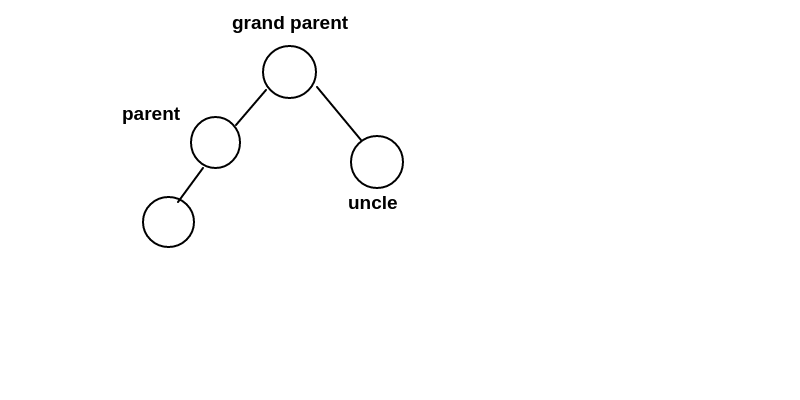
\includegraphics{img1.png}
\lstset{style=mystyle}
\begin{lstlisting}[language=C]
if((P[index] == LC[P[P[index]]]) && L[P[index]]==0 && L[P[P[index]]]==0 && L[RC[P[P[index]]]]==0){
    l2 = atomic_cmpxchg(&L[min],0,1); 
    l3 = atomic_cmpxchg(&L[mid],0,1);
    l4 = atomic_cmpxchg(&L[max],0,1);
\end{lstlisting}\\
In the above snippet of code we can see that first locks are checked normally then we use atomic operations to acquire locks. Since atomic operations are expensive, we don't bother using atomics once we know that a node is already locked. This is an optimisation done on locks.(See appendix for full code)\\
Every thread tries to acquire locks on four nodes and if it couldn't get the lock, the thread is stopped and the kernel is launched again in next iteration and the thread continues where it stopped. We use a while loop on host side which launches kernel and it stops only after all the nodes are inserted.The locks are acquired in the order of the node index to prevent live locks.\\
\centerline{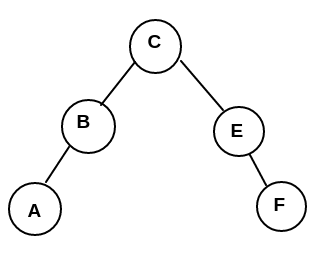
\includegraphics{img2.png}}
Assume situation where 2 threads are operating on nodes A and F. A tries to acquire locks on B,C,E and so do F. Now A acquires lock on B meanwhile F acquires lock on E. Since they cannto get locka on all 3 nodes they halt and same thing might repeat in the next iteration also. To prevent such situation we acquire locks in the order of node indices. Hence both threads first try to get lock on one of nodes and only one succeeds and other thread halts.



\chapter{Experimental Evaluation}

The code is ran on laptop with NVIDIA Dual SLI GT650M graphic card and 2.6 Ghz processor. It has 8 cores.
Initially we tried testing the non parallel code on CPU and see the time it takes. A tree is created with 2 lakh nodes. A graph is plotted against the time taken and percentage of nodes inserted.\\
\centerline{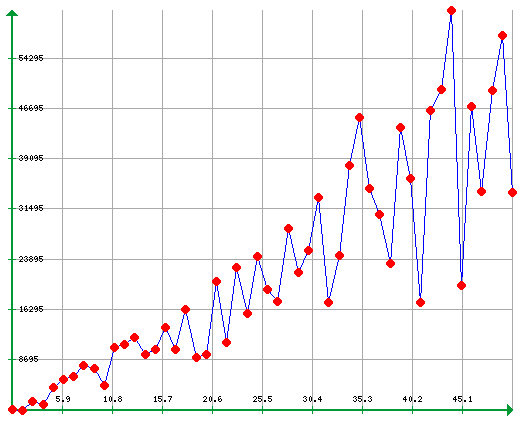
\includegraphics{Graph_seed3.png}}
X-axis is percentage of nodes added\\
Y-axis is time taken in micro seconds.\\
The time taken to create initial binary tree with 2 lakh nodes is 71,530 micro seconds.The graph is pretty expected since nodes are added one by one, as number of nodes increases time taken increases linearly. Some points have less time because it might have involved less number of rotations in that particular case.\\
Next the tree is implemented on GPU and similar graph is plotted.In this case initial tree is created on CPU with 1 lakh nodes and it is sent to the kernel. There nodes are added. The average time taken to create tree on CPU is 70023 micro seconds.This time graph is unexpected.There is a sudden rise in the time taken on GPU at 10-15\%. The reason is not known yet.\\
\centerline{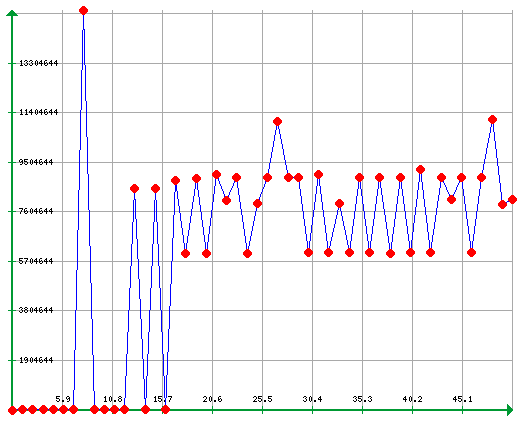
\includegraphics{Graph_gpu.png}}\\

\chapter{Related Work}
Synchrobench[2] have implemented a benchmark suite where you can test different synchronization techniques on data structures. They have implemented RB-Trees parallelly on CPU using transactional memory operations. You can different statistics like number of nodes inserted in a thread, number locks acquired by a thread, number of values read and written. But GPU has high computing power than CPU. SO many tried implementing parallel graph algorithms on GPU. Algorithms like BFS, SSSP, and MST yielded very good results. 
Rupesh Nasre, Martin Burtscher and Keshav Pingali have described how atomic free algorithms can be developed. They described how atomics can be avoided using barriers and exploiting the algebraic properties of algorithms. They describe 3 properties monotonicity, idem-potency and associativity which enables atomic free implementation.
\section{Conclusion}
At present, only insertion is done. Deletion has to be implemented. In the present implementation a single node is used as sentinel node. Because of this many threads which have only one sentinel node in common cannot do operations simultaneously.This decreases the performance. So different sentinel nodes can be used and performance can be checked. Since we are getting a step at 10-15\%of nodes, we can insert nodes by sending them in batches of 10\% of nodes.

\section{References}
\begin{enumerate}  
\item OpenCL learning: \newblock\\
https://www.fixstars.com/en/opencl/book/OpenCLProgrammingBook/contents/
\item Vincent Gramoli, More than you ever wanted to know about synchronisation\\
PPoPP 2015 Proceedings of the 20th ACM SIGPLAN Symposium on Principles and Practice of Parallel Programming
Pages 1-10 
ACM New York, NY, USA 2015 
\item Introduction to Algorithms Book, Thomas H.Coremen, Charles E. Leiserson, Ronald R. Rivest, Clifford Stein
\item Large-Scale Graph Processing Algorithms on the GPU\\
http://www.idav.ucdavis.edu/~yzhwang/gpugraph.pdf
\item Rupesh Nasre, Martin Burtscher, Keshav Pingali Atomic-free irregular computations on GPUs
Published in:Proceeding
GPGPU-6 Proceedings of the 6th Workshop on General Purpose Processor Using Graphics Processing Units
Pages 96-107 
ACM New York, NY, USA 2013 
\end{enumerate}

\appendix
\lstset{style=mystyle}

\chapter{RB-InsertFixup}
\begin{lstlisting}[language=C]
while(C[P[index]]){
		if( (P[index] == LC[P[P[index]]]) && L[P[index]]==0 && L[P[P[index]]]==0 && L[RC[P[P[index]]]]==0 ){
			__private int l1,l2,l3,l4;
			//l1 = atomic_cmpxchg(&L[index],0,1);
			a = P[index];
			b = P[P[index]];
			c = RC[P[P[index]]];
			if(a>b && a>c){
				max = a;
				if(b>c){
					mid = b;
					min = c;
				}
				else{
					mid = c;
					min = b;
				}
			}
			else if(a<b && a<c){
				min = a;
				if(b>c){
					max = b;
					mid = c;
				}
				else {
					max = c;
					mid = b;
				}
			}
			else {
				mid = a;
				if(b>c){
					max = b;
					min = c;
				}
				else{
					max = c;
					min = b;
				}
			}
			l2 = atomic_cmpxchg(&L[min],0,1); //take locks in increasing order of node indexes
			l3 = atomic_cmpxchg(&L[mid],0,1);
			l4 = atomic_cmpxchg(&L[max],0,1);
			//L[index]=1; L[P[index]]=1;  L[P[P[index]]]=1; L[RC[P[P[index]]]]=1;
			if(!l2 && !l3 && !l4){
				__private int z = c;
				if(C[z]){
					C[P[index]] = 0;
					C[z] = 0;
					C[P[P[index]]] = 1;
					__private int temp;
					temp = index;
					index = P[P[index]];
					L[temp]=0; L[P[temp]]=0; L[RC[P[P[temp]]]]=0;
				}
				else {
					if(index == RC[P[index]]){
						index = P[index];
						leftRotate(RC,LC,P,index,R);
					}
					C[P[index]] = 0;
					C[P[P[index]]] = 1;
					rightRotate(RC,LC,P,P[P[index]],R);
					L[index]=0; L[P[index]]=0;  L[RC[P[index]]]=0; L[RC[RC[P[index]]]]=0;
					return 0;
				}	
			}
			else{
				if(l2==0)L[min] = 0; //release locks acquired by this thread because it cant enter critical section
				if(l3==0)L[mid] = 0;
				if(l4==0)L[max] = 0;
				TL[base] = index;
				return 2;	
			}
		}
		else if( L[P[index]]==0 && L[P[P[index]]]==0 && L[LC[P[P[index]]]]==0 ){
			__private int l1,l2,l3,l4;
			//l1 = atomic_cmpxchg(&L[index],0,1);
			a = P[index];
			b = P[P[index]];
			c = LC[P[P[index]]];
			if(a>b && a>c){
				max = a;
				if(b>c){
					mid = b;
					min = c;
				}
				else{
					mid = c;
					min = b;
				}
			}
			else if(a<b && a<c){
				min = a;
				if(b>c){
					max = b;
					mid = c;
				}
				else {
					max = c;
					mid = b;
				}
			}
			else {
				mid = a;
				if(b>c){
					max = b;
					min = c;
				}
				else{
					max = c;
					min = b;
				}
			}
			l2 = atomic_cmpxchg(&L[min],0,1);
			l3 = atomic_cmpxchg(&L[mid],0,1);
			l4 = atomic_cmpxchg(&L[max],0,1);
			//L[index]=1; L[P[index]]=1;  L[P[P[index]]]=1; L[LC[P[P[index]]]]=1;
			if( !l2 && !l3 && !l4){
				__private int z = c;
				if(C[z]){
					C[P[index]] = 0;
					C[z] = 0;
					C[P[P[index]]] = 1;
					__private int temp;
					temp = index;
					index = P[P[index]];
					L[temp]=0; L[P[temp]]=0; L[LC[P[P[temp]]]]=0;
				}
				else {
					if(index == LC[P[index]]){
						index = P[index];
						rightRotate(RC,LC,P,index,R);
					}
					C[P[index]] = 0;
					C[P[P[index]]] = 1;
					leftRotate(RC,LC,P,P[P[index]],R);
					L[index]=0; L[P[index]]=0;  L[LC[P[index]]]=0; L[LC[LC[P[index]]]]=0;
					return 0;
				}
			}
			else{
				if(l2==0)L[min] = 0;
				if(l3==0)L[mid] = 0;
				if(l4==0)L[max] = 0; 
				TL[base] = index;
				return 2;
			}
		}	
}
C[R[0]] = 0;
L[index] = 0;
return 0;
\end{lstlisting}

\chapter{Right Rotate}
\lstset{style=mystyle}
 \begin{lstlisting}[language=C]
 x = LC[y];
	LC[y] = RC[x];
	if( RC[x] != 0)
		P[RC[x]] = y;
	P[x] = P[y];
	if(P[y] == 0){
		P[x] = 0;
		R[0] = x;  //making this node as root
		}
	else if(y == LC[P[y]])
		LC[P[y]] = x;
	else RC[P[y]] = x;
	RC[x] = y;
	P[y] = x;
 \end{lstlisting}
Left rotate is similar with right and left interchanged.
\end{document}
